\section{Eletrônica}
\par A solução de eletrônica do projeto consiste em garantir todo o funcionamento eletrônico do projeto, que é composto pelas áreas: telemetria, sensoriamento e controle do abastecimento e ignição do foguete.
\par Como o principal objetivo do projeto é construir um sistema de controle e monitoramento do foguete que permita isso ser feito a uma distancia segura, foi pensado em uma solução envolvendo telemetria tanto para colher os dados quanto para enviar sinais de comando. Para melhor detalhamento do projeto na parte de hardware a figura \ref{fig:Diagrama de Blocos} no apêndice \ref{Diagrama de blocos do sistema} resume bem a solução proposta.

%%\begin{center}
%%\begin{figure}[H]
%%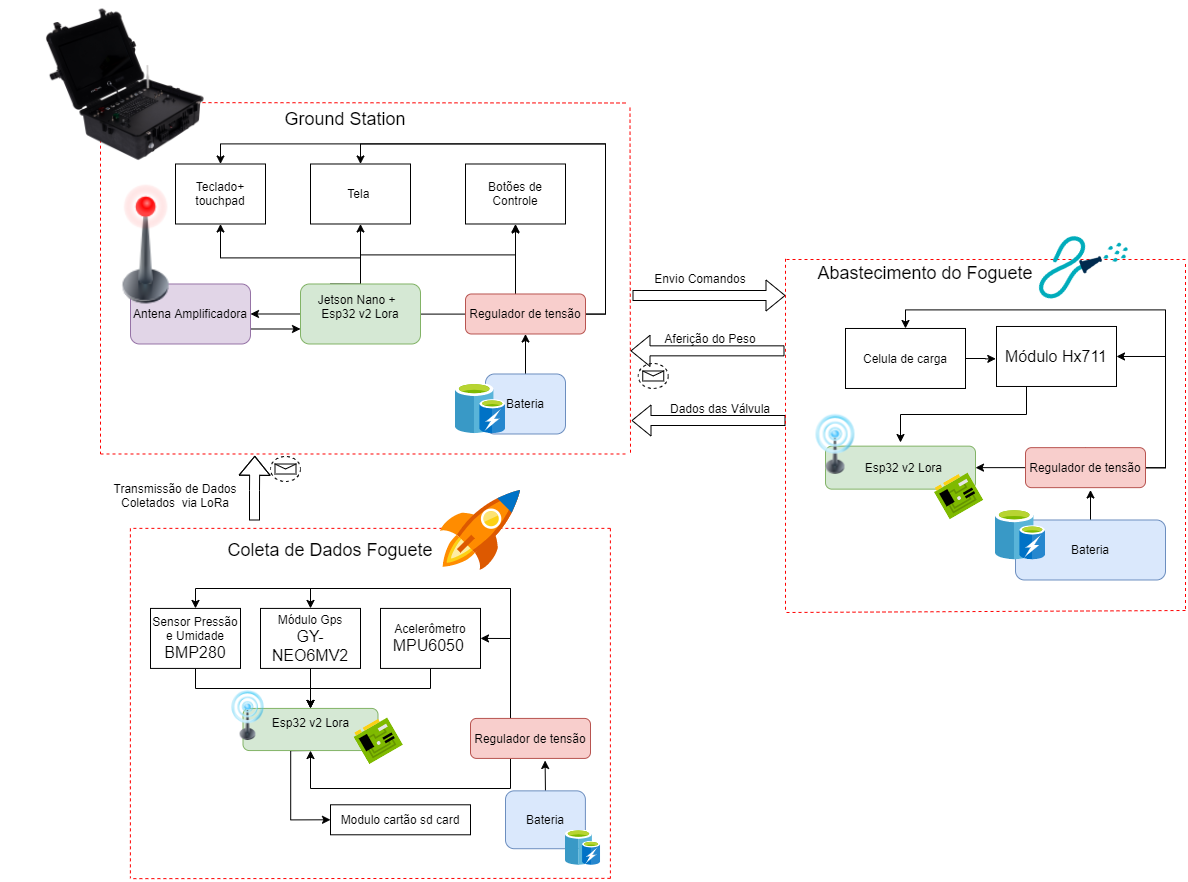
\includegraphics[scale=0.4]{editaveis/solucao/eletronica/diagrama pi2 (2).png}
%%  \caption{Diagrama de blocos do projeto.}
%%  \label{fig:Diagrama de Blocos}
%%\end{figure}
%%\end{center}

\subsection{Telemetria}
\par É um processo remoto de aquisição ou envio de dados, ou seja, é utilizado para medir, rastrear ou até mesmo controlar à distancia alguma coisa. Esse processo é feito geralmente por um sistema de comunicação sem fio como por exemplo por rádio frequência ou via satélite. \cite{Telemetria_AERONALTICA}.
\par Atualmente,  a telemetria está presente em diversos ramos da vida cotidiana do ser humano: na apuração das informações de um automóvel, no controle meteorológico, na agricultura e em outras diversas atividades.Para o projeto proposto, entende-se que o uso da telemetria em tempo real é extremamente vantajoso para a aquisição de dados durante o voo do foguete e para o controle autônomo do seu abastecimento/ignição.
\par Como requisito de segurança, é necessário fazer o controle  do foguete à distância. O recomendado pelas regras da LASC, competição a qual o cliente pretende participar, é uma distância mínima de 500m (lembrando que o foguete pode atingir uma altura de voo de aproximadamente 1km). Ou seja, fazer a aquisição de dados e o controle de abastecimento e ignição via cabo seria muito dispendioso, ou mesmo inviável, sujeito a maiores riscos de falhas, ou ficando na dependência de coletar os dados armazenados na memória do foguete somente após sua recuperação. Por essas razões, entende-se que é necessário realizar a telemetria em tempo real. Para melhor entendimento, na figura \ref{fig:Diagrama lançamento}   encontra-se o esquemático de um lançamento de foguete.
\begin{figure}[!htb]
\centering
\includegraphics[scale=0.4]{figuras/LANÇAMENTO.png}
\caption{Diagrama do Lançamento.}
{\footnotesize Fonte: Elaborado pelo autor.}
\label{fig:Diagrama lançamento}
\end{figure}

\par Como trata-se de uma função específica, o controle à distância e a aquisição de dados do pré-lançamento, do lançamento, do apogeu até a chegada do foguete no chão, é necessário compreender o problema e levantar requisitos para escolher a melhor forma de fazer a telemetria do projeto.
\par Foram analisados diversas formas de fazer a telemetria, entre elas estão: a telemetria feita por Radiofrequência, Lora, Wi-Fi, ZigBee, GPRS, Bluetooth, entre outras, analisando os seguintes requisitos: 
\begin{itemize}

\item Alcance;
\item Taxa de Transição de dados;
\item Protocolo de Comunicação;
\item Frequência dos Protocolos;
\item Potência de Transmissão; 
\item Interface de Dados;
\item Consumo.

\end{itemize}

\par Por fim, analisando diversos componentes, foi definido que a Placa Lora Esp32 da HELTEC figura \ref{fig:Placa Esp32 Lora } atende os requisitos do projeto citados acima, garantindo assim o funcionamento de qualidade do projeto, sendo que o principal motivo foi a distância alcançada pelo transmissor.

\begin{figure}[!htb]
\centering
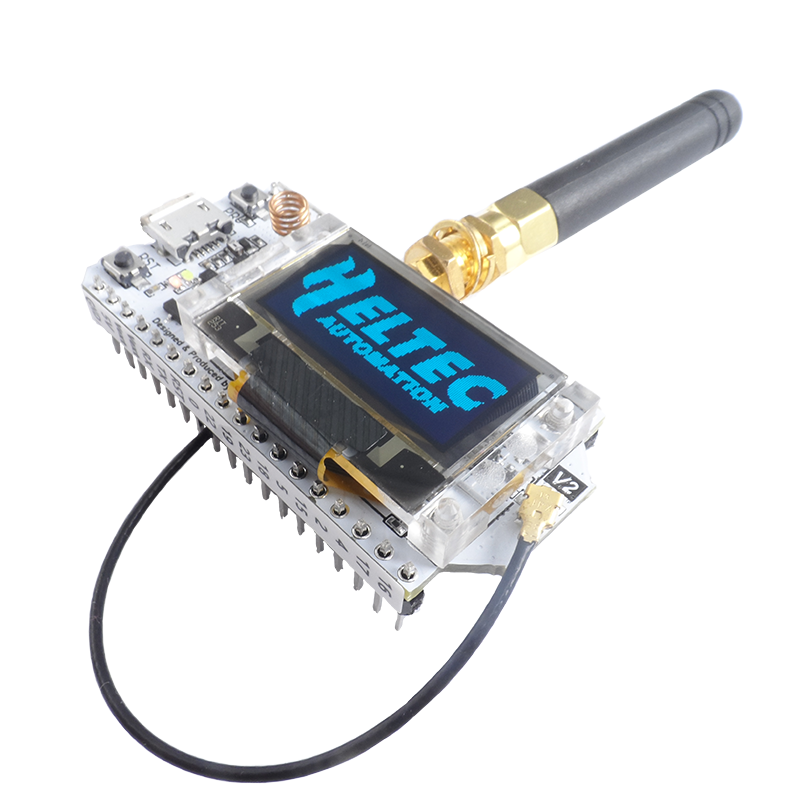
\includegraphics[scale=0.3]{figuras/SAM_0748_800X800.png}  
\caption{Placa Lora Esp32 da HELTEC.}
{\footnotesize Fonte:\cite{datasheet_ESP32}}
\label{fig:Placa Esp32 Lora }
\end{figure}
\par Contudo, como forma de garantir a integridade dos dados, foi pensado em ter um cartão MicroSD para gravação dos dados, evitando assim a perda de dados por falha na telemetria. 
\par Ainda será feito um levantamento do tamanho do pacote de dados que será gerado por cada sensor, a fim de obter uma análise completa do tamanho da informação que necessitará ser transmitida. Dependendo se a máxima taxa de dados transmitidos por segundo não conseguir suprir o tamanho do pacote gerado será necessário buscar alternativas para superar este problema como por exemplo adotar métodos de codificação\cite{Telemetria_AERONALTICA}. 

\subsection{Sensoriamento}

Sensores são dispositivos que possuem a função de detectar e responder com eficiência algum estímulo. Existem vários tipos de sensores que respondem à estímulos diferentes como por exemplo: calor, pressão, movimento, luz e outros. Depois que o sensor recebe o estímulo, a sua função é emitir um sinal que seja capaz de ser convertido e interpretado pelos outros dispositivos \cite{mattede_Sensores_blog2020}.

Definidos os requisitos do projeto, sabe-se que será necessário o uso de sensores e transdutores para a coleta de dados de altitude, velocidade e localização geográfica (GPS) do foguete, e também do peso do foguete durante o abastecimento na sua base de lançamento. Para tal, será utilizado apenas 3 sensores para obter essas 4 medidas.

\subsubsection{Altitude e Velocidade}

Para medição da altitude e velocidade do foguete durante o lançamento, foi escolhido o sensor de pressão e temperatura BMP280, visto na figura \ref{fig:sensor_pressao} \cite{datasheet_BMP280}.

\begin{figure}[H]
  \centering
  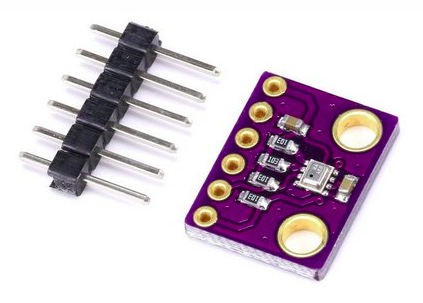
\includegraphics[scale=0.75]{figuras/BMP280.png}
  \caption{Sensor de pressão e temperatura BMP280 (Bosch). }
 { \footnotesize Fonte:\cite{figura_BMP280}} 
  \label{fig:sensor_pressao}
\end{figure}

Esse sensor mostrou-se o mais viável, pois, por meio da coleta dos dados de pressão atmosférica e temperatura, é possível, por meio de cálculos de altimetria, obter a altitude (em metros) do foguete em relação ao nível do mar durante o lançamento, conforme a equação \ref{eq_altitude_pressao}, que apresenta a relação da altitude com a variação de pressão atmosférica \cite{grusin_Tutorial_2018}.

    

\begin{equation}
Altitude = 44330 \times (1 - (\frac{P}{Po})^{\frac{1}{5.255}})
\label{eq_altitude_pressao}
\end{equation}


Onde Po é a pressão de linha de base (pode ser adotada a pressão a nível do mar ou pressão do local) em hPa e P é a pressão a obtida em hPa.

Logo, sabendo a altitude do foguete e obtendo a sua variação ao longo do tempo, este podendo ser medido pelo  \textit{clock} próprio do microcontrolador, é possível medir a velocidade do foguete em cada instante, por meio do cálculo da velocidade média, equação \ref{eq_vel_media}.

\begin{center}
\begin{equation}
\label{eq_vel_media}
V = \frac{\Delta S} {\Delta T}
\end{equation}
\end{center}

Onde V é a velocidade média em m/s, $\Delta$S é a variação de altitude em metros e $\Delta$T é a variação de tempo em segundos.

O sensor BMP280 realiza medições de pressão com precisão de $\pm$ 1 hPa e temperatura com precisão de $\pm 1 ^\circ C $. Com essa precisão, é possível realizar medições de altitude com margem de erro de  $\pm$ 1 metro, efetuando a leitura entre 300 e 1100 hPa, o que corresponde à faixa de altitude de +9000 à -500 m \cite{cia_BMP280_2017}.
Em relação aos sensores existente no mercado, o BMP280 foi o que melhor atendeu aos requisitos, pois ele é a versão mais atual e precisa dos modelos BMP180 e BM085, e também é de baixo consumo em relação aos sensores Mpx10dp e Mpx5700, possuindo melhor aplicabilidade.

\subsubsection{Localização Geográfica (GPS)}

A sigla GPS significa Global Positioning System, o que em português quer dizer Sistema de Posicionamento Global. É uma tecnologia que utiliza satélites e dispositivos para fornecer informações sobre a localização no globo terrestre \cite{fisica_GPS_2020}.
A localização GPS será utilizada para obter a posição geográfica do foguete após sua aterrissagem, podendo também fornecer as coordenadas ao longo do lançamento para determinar a trajetória percorrida pelo foguete.
Foi definido para tal função o GY-NEO6MV2 (Figura \ref{fig:moduloGPS}), um módulo GPS composto por duas partes, a antena, responsável por captar as informações provindas dos satélites e o sistema de controle, responsável pelo processamento dos dados obtidos, através do um microcontrolador interno NEO6 \cite{datasheet_GPS}.

\begin{figure}[H]
  \centering
  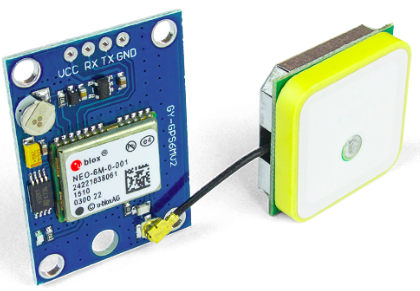
\includegraphics[scale=0.75]{figuras/moduloGPS.png}
  \caption{Módulo GPS GY-NEO6MV2 (uBlox). }
  {\footnotesize Fonte: \cite{figura_GPS}}
  \label{fig:moduloGPS}
\end{figure}

O módulo GPS GY-NEO6MV2 foi escolhido por ser de fácil utilização, realizando a comunicação através de comunicação serial, usando apenas 2 pinos (TX e RX), permitindo a comunicação com os mais diversos tipos de equipamentos e microcontroladores. Este apresenta um consumo de corrente em média de 45 mA, enquanto o módulo similar, VK2828U7G5LF, consome em média 50 mA.

\subsubsection{Peso do foguete}

Por meio do acompanhamento do peso do antes, durante e depois do abastecimento do foguete, será possível controlar e medir a quantidade de combustível contido em seu tanque. Para mensurar o peso do foguete, será utilizada uma célula de carga. 

Uma célula de carga é um transdutor de força que converte a carga que atua sobre ele em uma saída elétrica mensurável. Embora existam vários tipos, as células de carga baseadas em sensores de deformação e tensão são as mais usadas \cite{omega_celulacarga}. 

Neste projeto, foi escolhida a célula de carga de 50 kg, vide figura \ref{fig:celula_carga}, que atende o peso máximo do foguete, que é de 18.5 kg com o tanque de combustível cheio e 14.3 kg vazio (dados fornecidos pela Capital Rocket Team).

\begin{figure}[H]
  \centering
  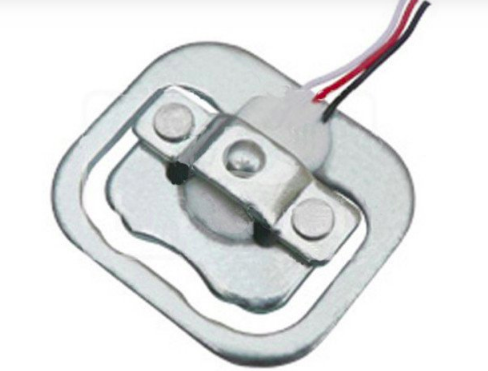
\includegraphics[scale=0.75]{figuras/celula_carga.png}
  \caption{Célula de carga - 50 kg.}
  {\footnotesize Fonte: \cite{figura_celula}} 
  \label{fig:celula_carga}
\end{figure}

Este é um sensor de carga de meia-ponte, amplamente utilizado em balanças. Quando a meia-ponte é esticada, é enviado um sinal elétrico através de um fio. É possível utilizar vários sensores de carga simultaneamente para aumentar a capacidade.
Como o sinal enviado pelo transdutor é elétrico, precisa-se de um módulo conversor, que fará a conversão do sinal elétrico em sinal digital para possibilitar a leitura dos dados pelo microcontrolador. Para isto, será usado o módulo conversor HX711, figura \ref{fig:conversorHX711}, um módulo amplificador e conversor HX711 de 24 bits, utilizado para amplificar o sinal de dispositivos como células de carga, fazendo a interligação entre essas células e o microcontrolador, por meio da comunicação SPI \cite{avia_HX711}.

\begin{figure}[H]
  \centering
  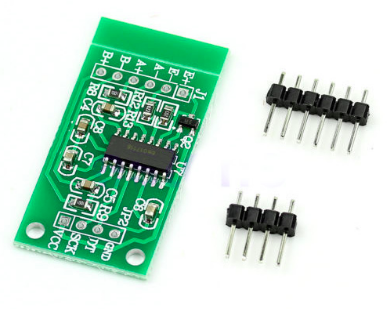
\includegraphics[scale=0.5]{figuras/conversorHX711.png}
  \caption{Célula de carga - 50 kg.}
  {\footnotesize Fonte: \cite{figura_HX711}} 
  \label{fig:conversorHX711}
\end{figure}

\subsubsection{Especificações dos sensores}
A tabela \ref{tab:sensores} apresenta os dados das principais especificações dos sensores citados acima.

\begin{center}
\begin{table}[H]
\centering
\begin{tabular}{ |m{2cm}|m{2cm}|m{2.5cm}|m{2.5cm}|m{2.5cm}|m{2.5cm}| } 
\hline

\textbf{ Sensor }&\begin{center}
\textbf{ Tensão de Operação} \end{center}& \textbf{Consumo de corrente }& \textbf{Comunicação} & \begin{center}\textbf{Taxa de transmissão} \end{center} & \begin{center}\textbf{Formato dos Dados}\end{center}\\ 
 \hline
 
 BMP280 & 1.71 - 3.6V & 3.6 $\micro$A @ 1 Hz (umidade, pressão e temperatura) & 
I2C e SPI & I2C (até 3.4 MHz e SPI (3 e 4 fios, até 10 MHz) & unsigned 20-bit (pressão e temperatura) unsigned 16-bit (umidade)\\
  \hline
Célula de carga 50kg & 5 -10V & Resistência de entrada e saída ($\ohm$): 1000 ± 50 & - & - & - \\
  \hline
 Módulo Hx711 & 4.8 - 5.5V & 1.5mA & SPI & 10 - 80 MHz & 24 bits em complemento de 2 \\ 
  \hline
 Módulo GPS GY-NEO6MV2 & 3 - 5V & 10mA – 100 mA & Serial UART e SPI & 9600 bps (UART baud rate) e 100 kbit/s & - \\ 
 \hline 

\end{tabular}
\caption{Especificações principais dos componentes do sensoriamento.}
\label{tab:sensores}
\end{table}
\end{center}


\subsection{Central de controle}

A central de controle será o ponto de acesso do usuário com os dados e comandos vindos da base de lançamento e do foguete. Um exemplo de estação pode ser visto na figura \ref{fig:DroneStation}. 

\begin{figure}[H]
  \centering
  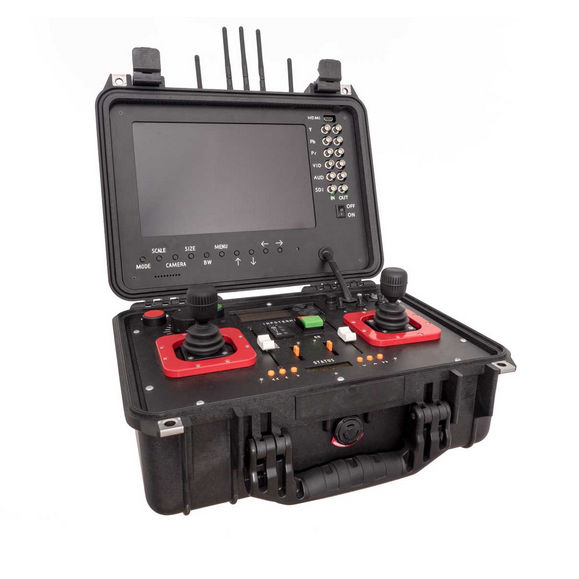
\includegraphics[scale=0.9]{figuras/DroneGroundStation.jpg}
  \caption{Estação de controle de solo.}
  {\footnotesize Fonte : \cite{AeroExpo}} 
  \label{fig:DroneStation}
\end{figure}


A solução proposta para essa interface do usuário foi seguindo esse modelo de maleta onde teria uma tela, um teclado e dois botões, sendo o primeiro para acionamento da ignição e um segundo para interromper os processos em caso de emergência.

\subsubsection{Interface do usuário}

A tela escolhida pode ser vista na figura \ref{fig:Tela}, esta tela possui um tamanho de 9 polegadas e uma resolução máxima de 1600x1200. 


\begin{figure}[H]
  \centering
  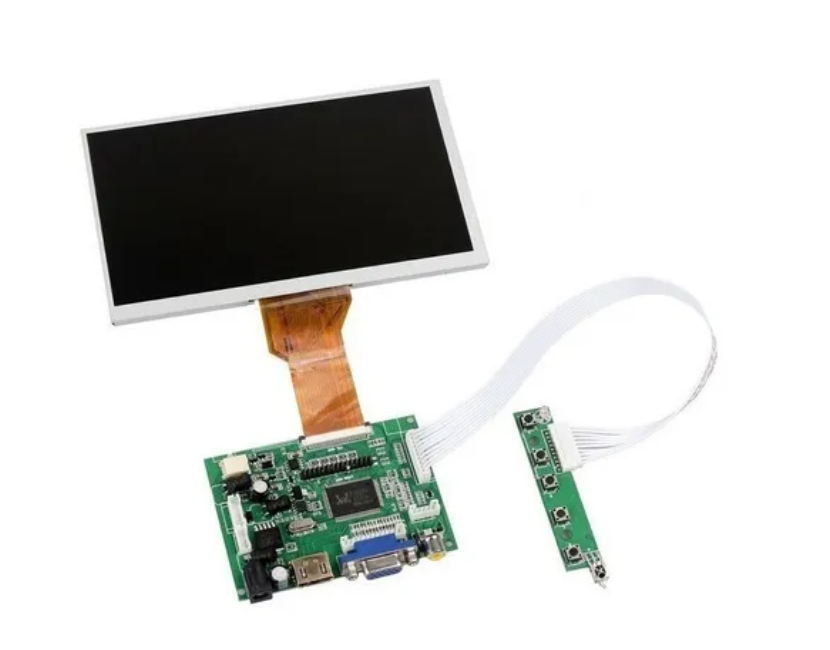
\includegraphics[scale=0.7]{figuras/TELAPI2.png}
  \caption{Tela da interface do usuário. }
  {\footnotesize Fonte : \cite{figura_Tela} } 
  \label{fig:Tela}
\end{figure}

Para a chegada dessa definição, pesquisas foram feitas e percebeu-se que geralmente telas menores, cinco e sete polegadas, possuem sensibilidade ao toque o que além de não agregar mais valor em nosso produto, dificultaria no dimensionamento da bateria dado a maior necessidade de potencia desse tipo de tela. Outro ponto levado em consideração é a questão da troca que existe entre o tamanho da tela e seu gasto energético. Precisava-se de uma tela grande o suficiente para a boa visualização dos dados, porém que fosse portátil e que consumisse pouca carga da bateria. Assim a escolha da tela com as características mencionadas anteriormente é justificada.

Para que o usuário interaja com essa tela, foi pensado em dois tipos de soluções. A primeira seria colocar todos os comandos em botões e chaves, e a segunda realizar os comandos por meio de um mini teclado. Optou-se pelo o uso do teclado, devido a possibilidade de maior interatividade com a aplicação de software e facilidade para futuras atualizações no projeto. 

O modelo de teclado portátil escolhido pode ser visto na figura  \ref{fig:Teclado}. Esse teclado possui dimensões de 200x126x6,2 mm e um peso de 200g.

Porém, em conversa com os nossos  \textit{stakeholders}, chegou-se à conclusão que um botão para a ignição e um botão em caso de falha seriam necessários, devido a possibilidade de acontecimento de falhas no processo de lançamento. Assim, esses dois botões também serão integrados à nossa solução.



\begin{figure}[H]
  \centering
  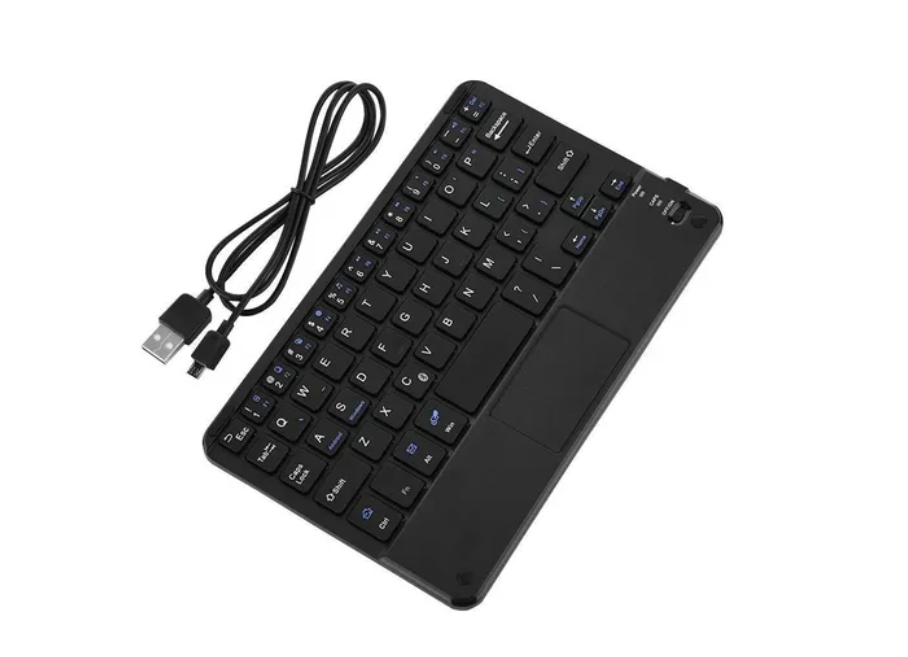
\includegraphics[scale=0.5]{figuras/TecladoPI2.png}
  \caption{Teclado da interface do usuário.}
  {\footnotesize Fonte : \cite{figura_Teclado}} 
  \label{fig:Teclado}
\end{figure}

\subsubsection{ \textit{Single Board Computer}}

Para a melhor escolha da placa utilizada no projeto, foi montada a seguinte tabela, na figura \ref{fig:comparacaoMicro}. Essa tabela foi levada aos grupos de software e de energia para o debate entre capacidade de processamento e custo energético.

\begin{figure}[H]
  \centering
  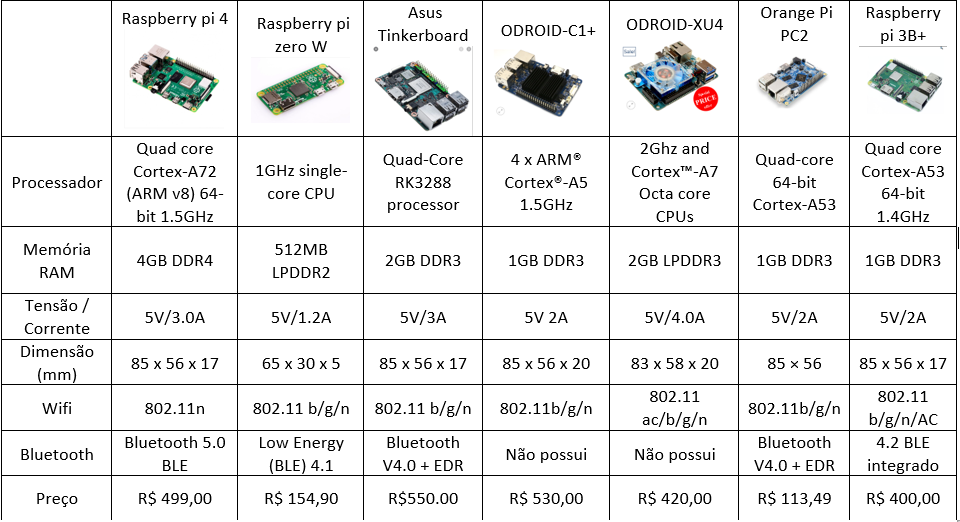
\includegraphics[scale=0.8]{figuras/SBCcomparacao.png}
  \caption{Tabela de comparação de single board computers. Fonte : Autor } 
  \label{fig:comparacaoMicro}
\end{figure}

Após algumas reuniões, ficou decidido que se usaria a raspberry pi 3B+ no projeto. Porém, conforme as  \textit{sprints} foram passando, percebemos juntamente com o grupo de software que seria necessário mais capacidade de processamento para os algoritmos que seriam implementados. Um novo alinhamento geral foi feito e a escolha que melhor atenderia essa demanda de processamento seria o uso de uma Jetson Nano Developer Kit da Nvidia, mostrado na figura \ref{fig:Nvidea}. 

\begin{figure}[H]
  \centering
  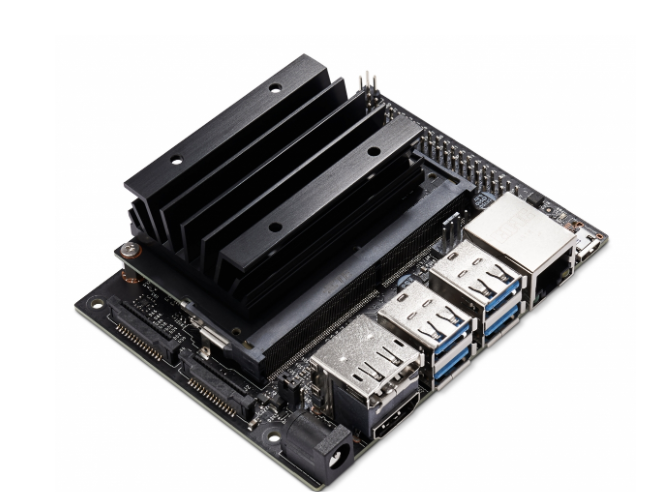
\includegraphics[scale=0.8]{figuras/NvideaPI2.png}
  \caption{Nvidea Jetson Nano Developer Kit. } 
  {\footnotesize Fonte : \cite{Nvidia_Nano} } 
  \label{fig:Nvidea}
\end{figure}

Apesar do detrimento causado no dimensionamento da bateria, essa placa foi escolhida devido a sua capacidade de processamento de algoritmos de  \textit{machine learning}, assim suprindo a demanda encaminhada pela equipe de software.